%&latex
\documentclass[12pt]{article}
\usepackage{amsthm,amsmath}
\usepackage{graphicx,psfrag,epsf}
\usepackage{enumerate}
\usepackage{natbib}
\usepackage{url} % not crucial - just used below for the URL
\usepackage{amsthm,amsmath}
\usepackage[utf8]{inputenc}

%\pdfminorversion=4
% NOTE: To produce blinded version, replace "0" with "1" below.
\newcommand{\blind}{1}

% DON'T change margins - should be 1 inch all around.
\addtolength{\oddsidemargin}{-.5in}%
\addtolength{\evensidemargin}{-.5in}%
\addtolength{\textwidth}{1in}%
\addtolength{\textheight}{1.3in}%
\addtolength{\topmargin}{-.8in}%


\begin{document}

%\bibliographystyle{natbib}

\def\spacingset#1{\renewcommand{\baselinestretch}%
{#1}\small\normalsize} \spacingset{1}


%%%%%%%%%%%%%%%%%%%%%%%%%%%%%%%%%%%%%%%%%%%%%%%%%%%%%%%%%%%%%%%%%%%%%%%%%%%%%%

\if0\blind
{
  \title{\bf Promoting analysis reproducibility with accessibility: An example in evolutionary biology}
  \author{Luna L. Sanchez Reyes\thanks{
    The authors gratefully acknowledge "Sustaining the Open Tree of Life", NSF ABI No. 1759838, and ABI No. 1759846.}\hspace{.2cm}\\
    School of Natural Sciences, University of California, Merced\\
    and \\
    Emily Jane McTavish \\
    School of Natural Sciences, University of California, Merced}
  \maketitle
} \fi

\if1\blind
{
  \bigskip
  \bigskip
  \bigskip
  \begin{center}
    {\LARGE\bf Promoting analysis reproducibility with accessibility: An example in evolutionary biology}
\end{center}
  \medskip
} \fi

\bigskip
\begin{abstract}
Reproducibility is essential for scientific development. Efforts
to increase scientific reproducibility have focused on increasing availability
of code and data. However, availability does not imply accessibility, and the latter
is infrequently addressed, even if it is key to achieve full workflow automatization
and reproducibility. Using an example in evolutionary biology, we identify factors
that have specifically affected accessibility in
the natural sciences, and ways researchers can address this to ensure reproducible
and automatic workflows.
The Open Tree of Life project (OpenTree) has developed a platform that facilitates
availability of results from evolutionary biology research. However, baseline
computational knowledge and skills required to
access scientific results are often not found among target users. While documentation
is available, it is often written using highly specialized language that is also
 inaccessible for the average target user.
We identified a set of principles to improve accessibility of OpenTree scientific data,
implement them in a tutorial, and elaborate on their general application to code and
documentation of scientific workflows.



\end{abstract}

\noindent%
{\it Keywords:}  open science, education, R, phylogenetics, tutorials
\vfill

\newpage
\spacingset{1.45} % DON'T change the spacing!
\section*{Introduction}
\label{sec:intro}

Reproducibility --the extent to which consistent results are obtained when a scientific
research experiment is repeated (\cite{repdef2021})-- is a key aspect for the advancement
of science, as it constitutes a minimum standard that allows understanding scientific products
(methods, analysis, results),
to determine their reliability and generality, and eventually build up scientific
knowledge and applications based on those products
(\cite{king1995replication, peng2011reproducible, powers2019open}).
In the natural sciences, rates of reproducibility are low (\cite{ioannidis2005most, prinz2011believe}),
prompting concerns about a reproducibility crisis in the field (\cite{baker2016reproducibility}).
%%% The scientific community has united to incentivize cultural changes that will improve
%%% reproducibility rates long term, such as transparency, availability, and workflow
%%% automatization, to name a few (\cite{peng2015reproducibility}).
In response, the scientific community has been generating standards and incentivizing
cultural changes in an effort to improve reproducibility rates long term
(\cite{peng2015reproducibility, wilkinson2016fair}).
One standard that has received much attention is scientific availability, which
 we define as the property of research objects to be acquired, copied, analyzed,
  processed and/or reused, at no financial, legal or technical cost (\cite{arnold2019turing}),
   and with no geographic, demographic or temporal barriers (\cite{fecher2014open}).
In this paper, we argue that availability can not be fully achieved without accessibility (Box 1)
We identify factors that have particularly affected accessibility in
the natural sciences, and ways researchers can address them to ensure reproducible
and automatic scientific workflows.
% full workflow automatization and reproducibility in the natural sciences


\bigskip
\bigskip

\noindent\fbox{%
    \parbox{\textwidth}{%
    \textbf{Box 1. The role of accessibility to achieve full availability.}
      Availability is generally defined as the ability or potential of something
      to be used and accessed (\cite{availability2022cambridge}).
      Following this definition, accessibility is generally considered a synonym of availability.
      Yet, in practice, availability does not imply accessibility.
      One example we find really useful to practically differentiate the concepts of availability and accessibility
      is the "marshmallows in an office" story, which goes like this.
      A couple of brand new marshmallow bags remained in a common office area after
      a social gathering.
      The marshmallows were not claimed by anybody, so they were left in the common are,
      freely available to be taken or eaten by anyone in the office.
      Yet, the marshmallow bags stayed in the common area, unopened for days and even weeks.
      It was not until someone decided to open the bags and placed the marshmallows on a tray,
      that people started actually eating them. They were gone in a matter of hours.
      Scientific products are not sweet as marshmallows, but they are a coveted resource.
      While sharing, describing and documenting makes scientific products available,
      it does not necessarily makes them accessible. For example, documentation of an
      available scientific workflow might be written using expert language that is too foreign
      for a general audience to successfully reproduce the workflow. While some individuals might
      be able to invest the time to learn the expert language to successfully reproduce
      the workflow, this will not be the case for the majority, even if it is
      something that would be useful long term, the short term time investment
      is often too high for individuals to engage with it, making the workflow and its results
      effectively inaccessible and hence unavailable to the majority of the community.
    }%
}
\bigskip


To elaborate on our thesis, we use an example in evolutionary biology that focuses
on understanding the shared ancestry of organisms through phylogenetic trees, which provide the
basis to study and understand biological processes in an evolutionary context (\cite{dobzhansky1973nothing}).
As such, improving reproducibility and availability
in phylogenetic research is relevant for many aspects of biological research.
The Open Tree of Life project (OpenTree) has developed a platform that facilitates
availability of results from phylogenetic research, by standardizing and storing
phylogenetic data with the goal of synthesizing a single phylogenetic tree encompassing
all life (\cite{opentreeoflife2019synth}).
All data in OpenTree is open access and available programmatically through its many
Application Programming Interface (API) services (\cite{opentreeAPIs}).
Additionally, R packages (\cite{michonneau2016rotl}) and Python libraries
(\cite{mctavish2021opentree}) have been developed as wrappers for OpenTree API services
to make them available to a wider programming audience.
The R and Python OpenTree wrappers have been utilized by computer-literate individuals,
to seamlessly establish reproducible workflows to use and reuse expert phylogenetic
knowledge for biological research (\cite{sanchez2019datelife}) and education
(\cite{nguyen2020phylotastic, phylotasticedtools, galacticedtools}).

The OpenTree project demonstrates that efforts to increase availability for reproducibility
in phylogenetics have also increased baseline computational knowledge and skills
required in the field.
Baseline computational skill requirements are likely increasing across all natural sciences.
Computing is not traditionally a core skill taught to biologists and naturalists.
However, many students are now being trained in R as a statistics and data analysis environment.
In order for reproducible computational tools to be adopted for research, they
 need to be much more accessible for present and future researchers.
Data and code availability is a core requirement for reproducibility research
 (\cite{peng2011reproducible, sandve2013ten, powers2019open}).
However, the utility of data resources is limited by the technical challenges of accessing the data.
In order to motivate reproducible research, that gap needs to be bridged.
In this work we focus on improving accessibility of code examples and documentation.
In particular, we identify the necessity for documentation that is written down
 using language that is common to the target audience to facilitate examination,
  application, and adoption of code by the wider audience.

We present a set of principles to generate documentation that improves accessibility
 of code and documentation. We applied these principles to a series of tutorials
  and vignettes developed for the OpenTree project.

\section*{Identifying hurdles to accessibility}
\label{sec:identifying}

Good primary documentation for code describes general usage of individual functions,
 the components and variables a function can take, and it should be accompanied with
  function usage examples on how to apply it.
As opposed to code, primary documentation is written in natural language (i.e.,
 any known human language, e.g., English, Spanish, Chinese) and usually makes use
  of highly specialized computational jargon (computationally specific concepts,
   words, and phrases) as well as formal language, which often slows down or even
    obstructs examination, application, and adoption of code by external individuals.
Because primary documentation is considered a professional document, acceptance
 of the research by the scientific community could be reduced if a more informal
  language is used.
Vignettes and tutorials work as secondary pieces of documentation, that help to demonstrate
 additional cases of individual function usage, and showcase function associations
  that work for specific analysis workflows in more detail.
   While secondary documentation has become more common practice,
    it is still often generated using highly specialized language.

\section*{Addressing hurdles to accessibility: some principles}
\label{sec:addressing}

\subsubsection*{a. Demonstrate integration of function usage with motivating examples}

We examined available primary documentation for the OpenTree API R wrapper (the package `rotl`),
and designed a workflow that visits as many functions as possible, and demonstrate
uses commonly requested by OpenTree users that are not demonstrated elsewhere.
By framing the function workflow using highly requested uses, the documentation acquires a
narrative arc that is easier to follow and remember by users. This facilitates the translation
of functions to specific use cases in biology.

For the tutorial demonstrated here, we used the commonly requested use case of obtaining
a phylogenetic tree for all lineages within a specific taxonomic rank.

\subsubsection*{b. Demonstrate errors and warnings thoroughly}

Primary documentation focuses on demonstrating usage function with examples that
work seamlessly, without errors. We argue that the opposite is needed to support
user adoption of reproducible workflows: demonstrate examples that do not work
as expected and exemplify ways to address them (Figure \ref{fig:first}).
We identify inputs that would give
a wide range of warnings and errors, focusing on demonstrating these cases. This
helps users to not be afraid of errors and warnings, but instead to use them to
their advantage.
We also identify effects of warnings and errors downstream of the workflow.

We identify ways to evaluate inputs to know if they will produce an error, and design
alternatives on what to do when faced with an error or warning, and demonstrate
these alternatives.
One of the most essential skills in programming is interpreting and moving forward
from errors.
Many finely honed tutorials do not trigger errors, which precludes helping students
to develop the tools to understand and address errors when they do encounter them,
as they inevitably will.
On our tutorial, we focus on explaining the meaning and downstream coof warnings and errors, and
 showcase ways to detect them before they are triggered (i.e., before using an input
  that would elicit a warning or error). This has two pedagogical benefits:
1) it provides users/students with the means to troubleshoot their own warnings and erros, and
2) it allows users/students to understand with more depth what the function is doing.

We designed ways to access the different elements of the outputs.

\begin{figure}
\begin{center}
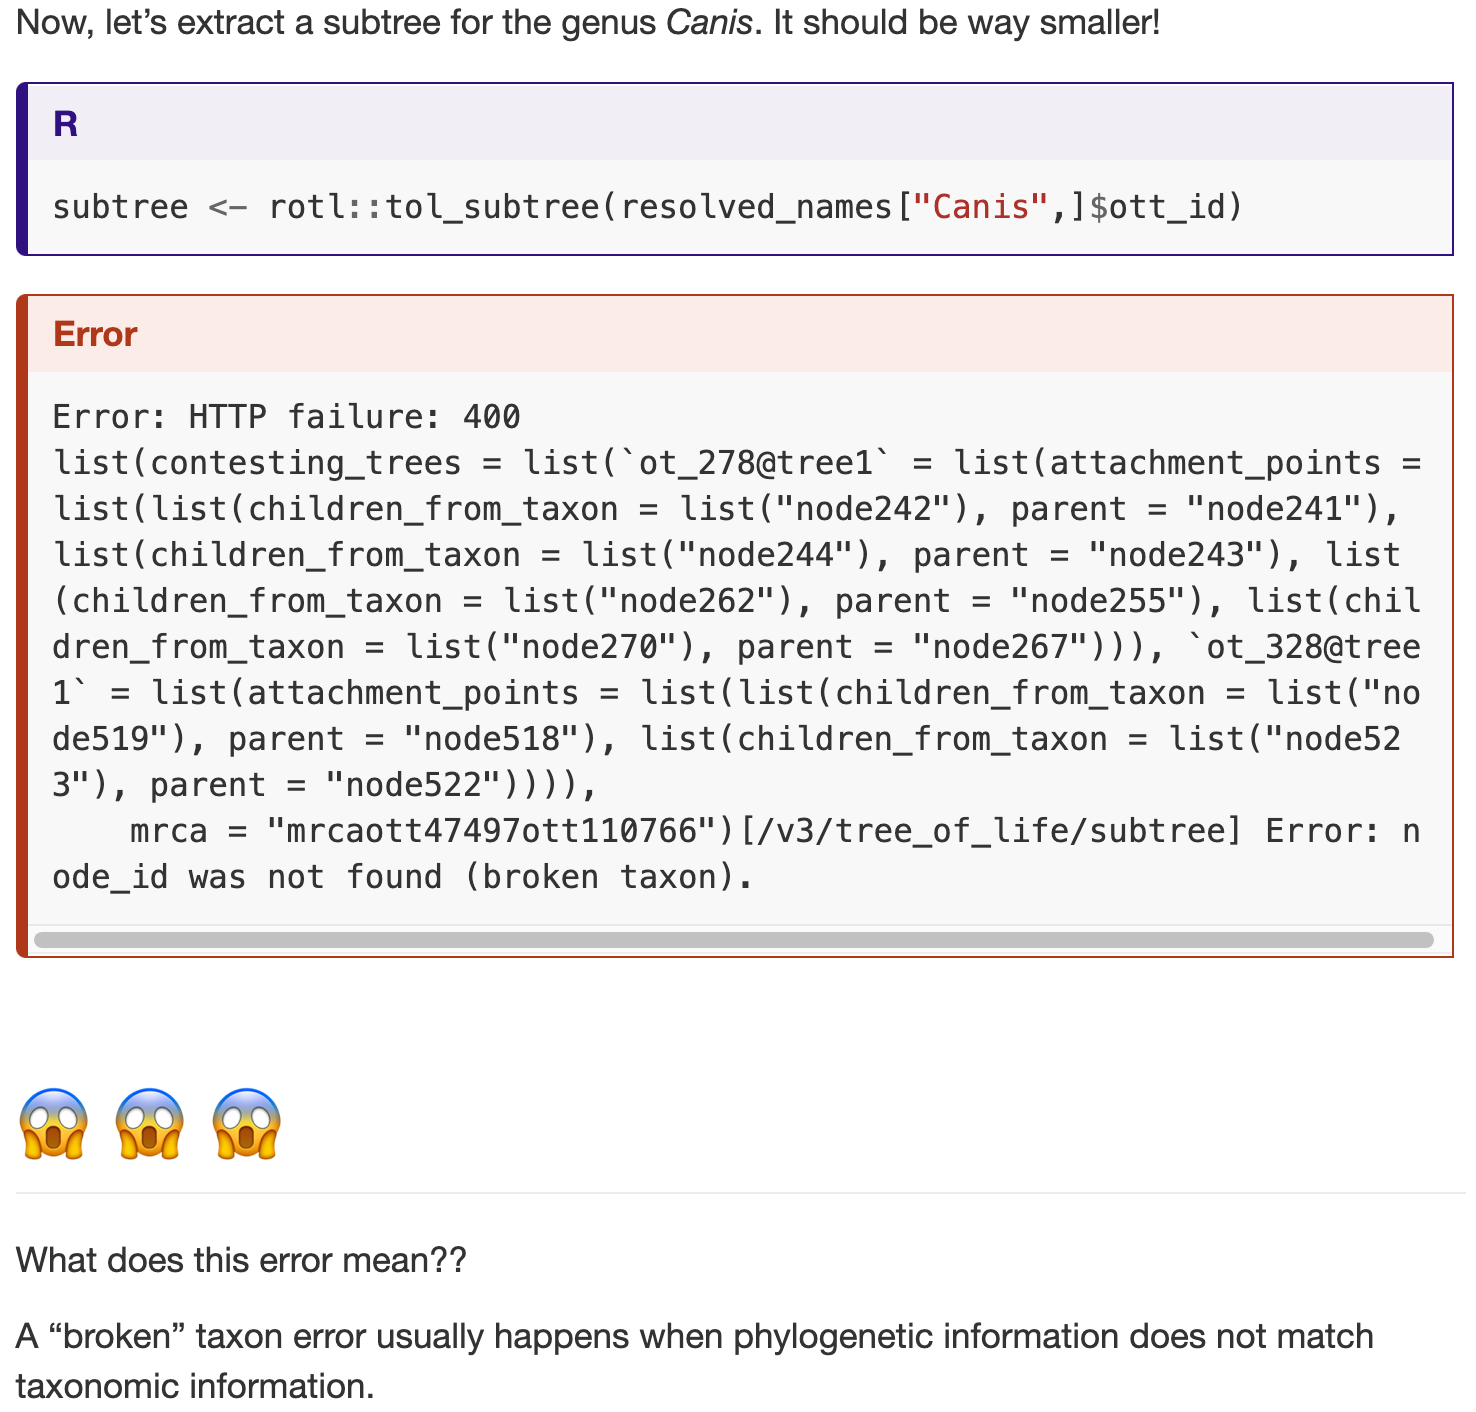
\includegraphics[width=3in]{fig1.png}
\end{center}
\caption{Snapshot of a section of the tutorial website, where we demonstrate a common error. \label{fig:first}}
\end{figure}

\subsubsection*{c. Avoid jargon and expert language}

Besides avoiding formal language, and incorporating elements of pop culture, such as picture
character icons known as "emojis", to make the language more familiar to a
broader target audience (see Figure \ref{fig:first}), we made an effort to specifically
complement the primary documentation by identifying
computational concepts that were assumed or were not explained in depth.
We vetted the tutorials with an audience on workshops as well as individual user.
We choose examples that are charismatic for the audience.
For example, when we presented the tutorial for a team specialized in Amphibians,
we tailored the examples using frogs and their allies.


\subsubsection*{d. Make it stable through time}

We published the tutorials on a public, free license, free of cost, and free for
use and reuse repository and persistent website (\cite{RopentreeTutorials, RopentreeTutorialsWebsite}).
The tutorial is available for the users to go back to it any time they need it,
and to be passed on to other users (Figure \ref{fig:second}).

\begin{figure}
\begin{center}
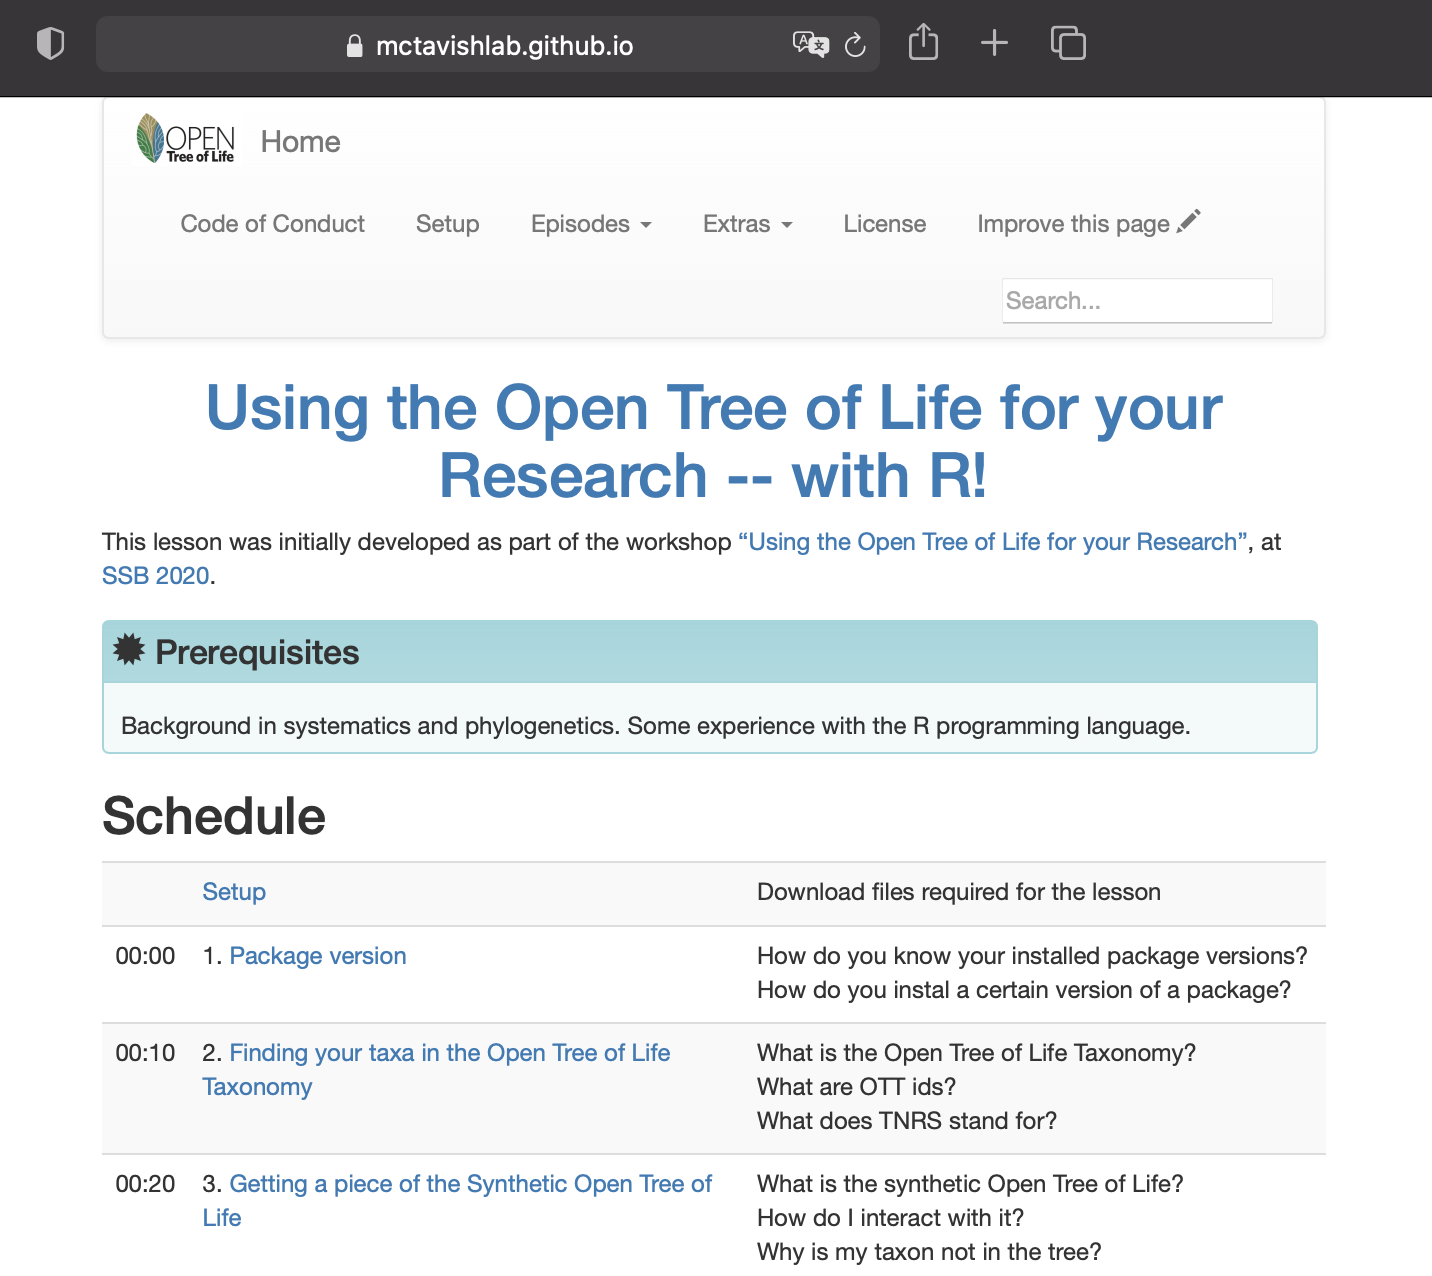
\includegraphics[width=3in]{fig2.png}
\end{center}
\caption{Snapshot of the home to our tutorial website, showing part of the schedule. \label{fig:second}}
\end{figure}

Following the carpentries, we created a main version of the tutorial that
is updated. Versions presented on workshops are a copy from the original repository,
and represent a stable and temporal snapshot of the functions and workflows presented
in the tutorial.

%%% \subsubsection*{5. The (now) classics of computational reproducibility}
%%%
%%% Provide all information on package version and system capabilities.
%%%
%%% > [name=Emily Jane McTavish]link to where/and how you did that

\section*{Conclusion}
\label{sec:conclusion}

Ultimately, the improvement of reproducibility rates in science long term depends
on our ability to intentionally integrate the subject of reproducibility in the
the curriculum for college students and aspiring researchers to develop the skills
necessary to create reproducible scientific workflows and materials.

Some universities have been incorporating the subject in their classes (see University
 of Washington and The National Institute for General Medical Sciences).
The focus has been on students to develop skills to document their work.
The principles identified and outlined here can be used to set learning goals and
 outcomes on new reproducibility syllabus.





We have received emails from senior researchers thanking us for this materials,
 and students have been able to engage using the packages with less hep from the PIs.

The principles to create tutorials described here facilitate adoption of software
 and analysis workflows among researchers at different academic levels, from undergrads
  to established researchers.
It will also help closing the gap between students that had access to computational
 resources (and computational training) from an early age and students that did not.
  Late access to computational resources and training can occur due to lack of
   economic resources, often occurring in households from underrepresented communities
    and minorities.
It can also be due to gender-biased parental and community pressures,
 in which male individuals are more often encouraged to perform activities related to computers,
  while female individuals are discouraged.
% How to balance software acceptance VS. adoption?
These principles can be used to aide not only in improving reproducibility practices,
 but also software adoption in the natural sciences.
%% Discuss: why address accessibility and not other aspects of reproducibility?


Making accessible reproducible workflows has several advantages:
save explanation/training time when analyses are run again by students and collaborators.
save research time for yourself when analyses are run again with more data, a different dataset, a different organism or biological model.
scientific efforts can build off of each other

\bigskip
\begin{center}
{\large\bf SUPPLEMENTARY MATERIAL}
\end{center}

\begin{description}

\item[Title:] Website and GitHub repository containing the complete teaching materials developed and demonstrated here.

\item[GitHub repository link:] \url{https://github.com/McTavishLab/R_OpenTree_tutorials}

\item[Website link:] \url{https://mctavishlab.github.io/R_OpenTree_tutorials}

\end{description}

\bibliographystyle{agsm}

\bibliography{Manuscript-bibliography}

\end{document}
